\documentclass[lettersize,journal]{IEEEtran}
\usepackage{amsmath,amsfonts}
\usepackage{algorithmic}
\usepackage{algorithm}
\usepackage{array}
\usepackage[caption=false,font=normalsize,labelfont=sf,textfont=sf]{subfig}
\usepackage{textcomp}
\usepackage{stfloats}
\usepackage{url}
\usepackage{verbatim}
\usepackage{graphicx}
\usepackage{cite}
\hyphenation{op-tical net-works semi-conduc-tor IEEE-Xplore}

\begin{document}

\title{Framework for Assurance of Emergent Behaviour for use in Autonomous Robotic Swarms}

\author{Author1\_Name, Author2\_Name, ...AuthorN\_Name,
\thanks{Author1 and Author2 are with the Department of Dep1\_Name (email: , )}
\thanks{AuthorN is with the Department of Dep2\_Name (email: )}}
%\thanks{Manuscript received April 19, 2021; revised August 16, 2021.}}
% The paper headers
\markboth{Journal of \LaTeX\ Class Files,~Vol.~14, No.~8, August~2021}%
{Shell \MakeLowercase{\textit{et al.}}: A Sample Article Using IEEEtran.cls for IEEE Journals}

%\IEEEpubid{0000--0000/00\$00.00~\copyright~2021 IEEE}
% Remember, if you use this you must call \IEEEpubidadjcol in the second
% column for its text to clear the IEEEpubid mark.

\maketitle

\begin{abstract}
	Abstract of the paper.
\end{abstract}

\begin{IEEEkeywords}
	Assurance, swarm robotics, trustworthiness, safety, transparency, ethics, autonomous systems
	%Swarm Robotics, Acceptability and Trust, Autonomous Agents
\end{IEEEkeywords}

\section{Introduction}\label{introduction}
The main contribution of this paper is a novel framework for assurance of emergent behaviour for use in autonomous robotic swarms based on the AMLAS, SACE* and SOCA* guidance (* under consideration). We illustrate the framework using a public cloakroom case study. 

%\\\noindent\textbf{\textit{[Author General Guidelines: please write as a paper not as a Guidance like AMLAS; Please do not use AERoS word]}}\\


\section{Background and Related Work}\label{background-relatedwork}

\subsection{Background}\label{background}

\subsubsection{Specification Challenges and Standards}
%\newline With respect to swarms, the overall behaviours of a swarm are not explicitly engineered in the system, but they are an emergent consequence of the interaction of individual agents with each other and the environment.
%This emergent functionality poses a challenge for specification. 
%\newline How do you ensure safety or any other extra-functional property of a swarm where the swarm’s behaviour is an “emergent” consequence of the interaction of individual agents with each other and their environment?
%Swarm behaviours:
%\newline Aggregation 
%\newline Coherent ad-hoc network
%\newline Information retrieval
%\newline Taxis towards pick up and delivery areas of boxes
%\newline Obstacle avoidance
%\newline Object organization
%
%\textit{IEEE P7001} standard describes measurable, testable levels of transparency for autonomous systems so that they can be objectively assessed and levels of compliance determined\cite{IEEE-P7001}. 
%This standard outlines five stakeholder groups, and for each group it explains the structure of the normative definitions of levels of transparency. 
%\textit{IEEE P7001} can be applied to assess the transparency of an existing system using a process of System Transparency Assessment, or to specify transparency requirements for a system prior to its implementation (System Transparency Specification).
%The 5 stakeholders are end users, general public and bystanders, safety certification agencies and auditors, incident/accident investigators, expert advisors.
%
%In service robotics, ISO 13482 covers the hazards presented by the robots and devices for applications in non-industrial environments for providing services. 
%ISO 23482-1 and ISO 23482-2 standards extend ISO 13482 with guidance and methods that can be used to test personal care robots.
%On the other hand, in the industrial sector, ISO 10218-1 and ISO 10218-2 provide safety requirements for industrial robots and their integration.
%Meanwhile, ISO/TS 15066 provides safety requirements for collaborative industrial robot systems and work environment. 
%Although these industry standards focus on ensuring safety of robots at the individual robot level, they do not ensure safety or any other extra-functional property at the swarm level, which is a limitation.
%
%This Figure shows a categorization of robots by ISO. 
%Identifying which robot category the individual robots of the cloakroom is important because different legal and regulatory requirements apply to different robot categories.
%The “service robot” contains most robot categories, except industrial robot. 
%These are: household robots, medical robots and personal care robots.
%The individual robots of the cloakroom better fit into the “mobile servant robots” category, which is a type of personal care robot under service robots.
%A mobile servant robot is a personal care robot capable of travelling to perform serving tasks in interaction with humans, e.g. handling objects or exchanging information [ISO 13482:2014, 3.14].
\vspace{2mm}

\subsubsection{Robotic Swarms}
%\noindent Autonomous
%\\ \noindent Large Number of agents (10+)
%\\ \noindent Relatively incapable individuals
%\\ \noindent Restrained Homogeneity
%\\ \noindent Minimal communication capabilities (Decentralised)
\vspace{2mm}

\subsubsection{Case Study}

\vspace{2mm}
\noindent\textbf{\textit{\newline[Author Guidelines: Please use the cloakroom case study to illustrate the framework in Section III. If the examples in cloakroom case study are not sufficient, other swarm use cases listed below can be considered.]}}

\paragraph{\textbf{Cloakroom}}
The case study describes a public cloakroom where swarm of robots assist customers looking to deposit their jackets at an event \cite{Jones2020}. 
It describes cases where customers are depositing jackets, handing a jacket to a robot for storing, and retrieval of jackets back to the customer. 

\paragraph{Other Swarm Use Cases}
\textbf{\\Fault detection, diagnosis and recovery – Monitoring fires in a natural environment}. Fault detection model shall be trained to high level of accuracy. Thresholds for fault tolerance shall be set appropriately such that misclassification of a fault is a rare event. An agent experiencing minor faults shall not be immediately removed, should the fault not impact the task at hand. \\
\textbf{\noindent Social swarm – Brainstorming at an event}. Humans follow robots which cluster based on input. Minimise blocking paths of other humans and agents. Maintain situational awareness of humans and agents in the environment. Before the task, provide a clear explanation of the steps of the activity. Clear guidance during the task. Provide information about how the swarm/robot works.

\noindent See research paper ``Mutual shaping in swarm robotics: User studies in fire and rescue, storage organization, and bridge inspection" \cite{Carrillo-Zapata2020}.

\subsection{Related Work}\label{relatedwork}

\subsubsection{Assurance of Machine Learning in Autonomous Systems (AMLAS)}
%\cite{Hawkins2021}
\textit{Assurance of Machine Learning for use in Autonomous Systems (AMLAS)} provides guidance on how to systematically integrate safety assurance into the development of machine learning components based on offline supervised learning \cite{AMLAS2021}. 
AMLAS provides an explicit and structured safety case that the system is safe to operate in its intended context of use. 
AMLAS contains six stages, and the assurance activities are performed in parallel to the development of machine learning component. 
The process is iterative by design and feedback is used to update previous stages. 

\subsubsection{Safety Assurance of Autonomous Systems in Complex Environments (SACE)}
\cite{SACE2022}

\subsubsection{Societal Acceptability of Autonomous Systems (SOCA)}
\cite{Porter2022,McDermid2021}

\section{Framework}\label{framework}

\subsection{Overview of Framework} \label{framework-overview}
%Simple algorithms are executed by individuals.
%These simple behaviours performed by large numbers of agents build to emergent behaviours.
%The adaptivity provided by emergence requires assurance. 
%
%Safety Assurance Process based on AMLAS targeting robotic swarms:
%Emergent behaviour
%Failure conditions that the output of an individual robot or a robot in the neighbourhood makes to potential swarm-level hazards.
%
%Scope of current study:
%Looking purely at inherent swarm qualities and the adaptation that stems from these.
%Developing individual behaviours which when combined create an adaptive emergence.
%Machine/Reinforcement Learning should not be considered at this time.
%We may expand to ML/RL for individuals. (Application of AMLAS to individuals once AMLAS has been applied to the swarm)
\vspace{2mm}

\subsection{Stage 1: EB Safety Assurance Scoping} \label{framework-stage1}
\noindent \textbf{\textit{[Lead:  WP1]}}\\
\noindent\textbf{\textit{[Author Guidelines: 900–1800 words / 1–2 pages (maximum); \\Format/structure: Describe adapted AMLAS activities, inputs and outputs using cloakroom case study examples. Activities: 1, 2; Inputs: A, B, C, D, F; Outputs: E, G]}}\\
See Fig.~\ref{amlas-a-stage1}
\begin{figure*}
	\centering
	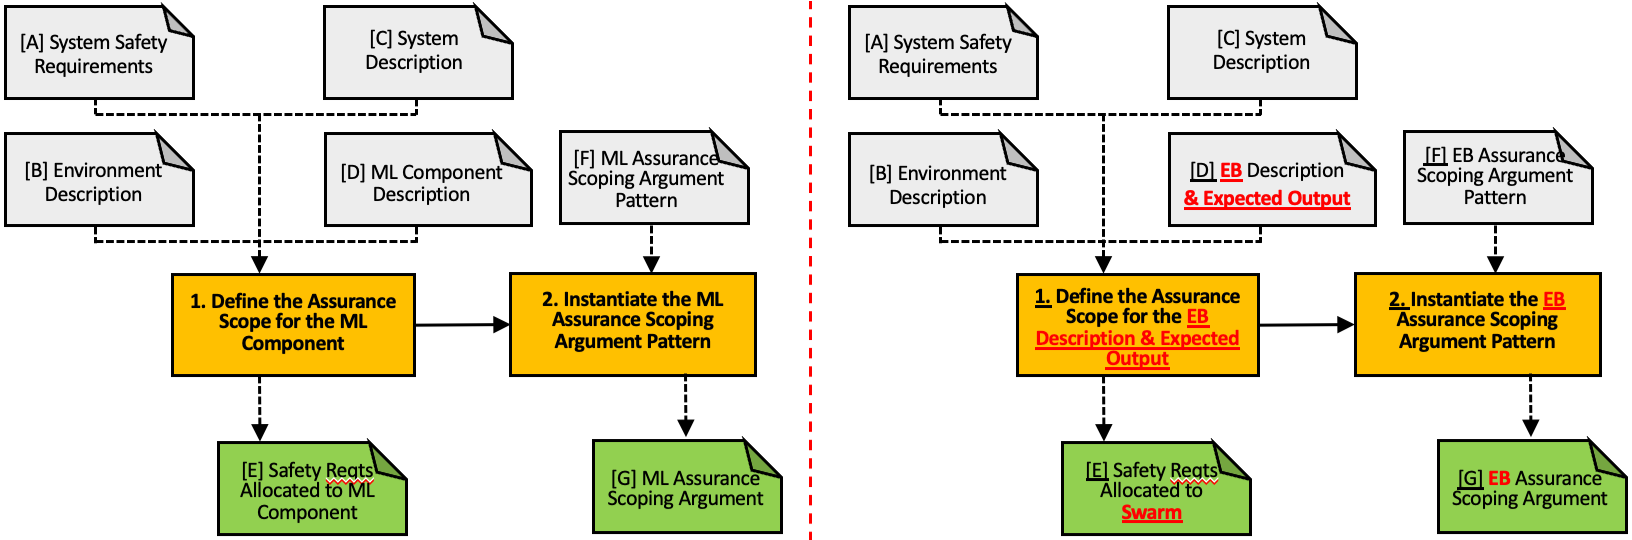
\includegraphics[width=1.0\textwidth]{figures/amlas-a-stage1.png}
	\caption{Adapted AMLAS emergent behaviour assurance scoping process (right).}
	\label{amlas-a-stage1}
\end{figure*}

\subsection{Stage 2: EB Safety Requirements Assurance} \label{framework-stage2}
\noindent \textbf{\textit{[Lead:  WP1; Other: WP2, WP3]}}\\ 
\noindent\textbf{\textit{[Author Guidelines: total 7 pages (maximum); \\Format/structure: Describe adapted AMLAS activities, inputs and outputs using cloakroom case study examples. \\
\noindent WP1 = (Activities: 3, 4, 5; Inputs: E, I; Outputs: H, J, K: 2700 words / 3 pages maximum))\\
\noindent WP2 = (List of Ethical Requirements and Description: 1800 words / 2 pages maximum)\\
\noindent WP3 = (List of Socio-Technical/Regulatory Requirements and Description: 1800 words / 2 pages maximum)]
}}\\

WP3
Sociotechnical Requirements Analysis for Autonomous Robotic Swarms
The focus of much work to date on the design of autonomous systems and specification techniques to assure safety in these systems has primarily been on developing technical aspects of assurance (Brundage et al., 2020). However, despite significant investments and efforts, getting technical safety assurance right has proved to be a challenging task (see, for instance, Karvonen et al., 2020; Thieme et al., 2021; Hernandez et al., 2021). The causes for problems are complex and varied and remain poorly understood. Simplistic claims that technical assurance will reduce risk to technological performance ignores the inherently sociotechnical nature of autonomous and intelligent systems: the fact that “all technologies are designed, developed, built, deployed, maintained, supervised, operated, and governed by people; and those people necessarily work within, and are shaped by, complex social, cultural, and organisational processes” makes assurance extremely complex (Macrae, 2021: 3; Pettersen Could, 2021; Reason, 1997). 



\newpage
\noindent \textbf{Stage 2 Requirements (Input H)}\\
\noindent \textbf{Cloakroom: Performance Requirements: }
\begin{center}
	\begin{tabular}{|p{7mm}|p{72mm}|}
		\hline
		& \textbf{Requirements for Faultless Operations} \\
		\hline
		RQ1.1 & The swarm \emph{shall} experience $<$ 1 low impact (V $<$ 0.5m/s) collisions across 1000 seconds of faultless operation. \\ 
		\hline
		RQ1.2 & The swarm \emph{shall} experience $<$ 1 high impact (V $>$ 0.5m/s) collisions across a day of faultless operation. \\ 
		\hline
        & \textbf{Requirements for Failure Modes (Graceful Degradation): } \\
        \hline
		RQ1.3 & The swarm \emph{shall} experience $<$ 10\% increase in low impact collisions across 1000 seconds of operation with 10\% injection of full communication fault to the swarm. \\
		\hline
		RQ1.4 & The swarm \emph{shall} experience $<$ 0.1\% increase in high impact collisions across a days operation with 10\% injection of full communication fault to the swarm.\\ 
		\hline
		RQ1.5 & The swarm \emph{shall} experience $<$ 10\% increase in low impact collisions across 1000 seconds of operation with 50\% injection of half-of-wheels motor faults to the swarm.\\
		\hline
		RQ1.6 & The swarm \emph{shall} experience $<$ 0.1\% increase in high impact collisions across a days operation with 50\% injection of half-of-wheels motor faults to the swarm.	\\	
		\hline
	    & \textbf{Requirements for Worst Case: } \\
	    \hline
		RQ1.7 & The swarm \emph{shall} experience $<$ 2 low impact (V $<$ 0.5m/s) collisions across 1000 seconds of faulty operation. \\			\hline	
		RQ1.8 & The swarm \emph{shall} experience $<$ 2 high impact (V $>$ 0.5m/s) collisions across a day of faulty operation.  \\		[1ex] 		
		\hline
	\end{tabular}
\end{center}

\noindent \textbf{Cloakroom: Adaptability Requirements: }
\begin{center}
	\begin{tabular}{|p{7mm}|p{72mm}|}
		\hline
		& \textbf{Requirements for Faultless Operations} \\
		\hline
		RQ2.1 & The Swarm \emph{shall} have $<$ 10\% of its agents stationary* outside of the delivery site at a given time.
		*Assumption: Agents are considered stationary once they have not moved for $>$ 10 seconds.
		 \\ 
		\hline
		RQ2.2 & All agents of the swarm \emph{shall} move at least every 100 seconds if outside of the delivery site. \\ 
		\hline
		& \textbf{Requirements for Failure Modes (Graceful Degradation): } \\
		\hline
		RQ2.3 & The swarm \emph{shall} experience $<$ 10\% increase in number of station agents at any given time with 50\% injection of half-of-wheels motor faults to the swarm. \\
		\hline
		RQ2.4 & The swarm agents \emph{shall} experience $<$ 10\% increase in stationary time with 50\% injection of half-of-wheels motor faults to the swarm.\\ 
		\hline
		RQ2.5 & The swarm \emph{shall} experience $<$ 10\% increase in number of station agents at any given time 10\% injection of full communication fault to the swarm.\\
		\hline
		RQ2.6 & The swarm agents \emph{shall} experience $<$ 10\% increase in stationary time 10\% injection of full communication fault to the swarm. \\	
		\hline
		& \textbf{Requirements for Worst Case: } \\
		\hline
		RQ2.7 & The Swarm \emph{shall} have $<$ 20\% of its agents stationary* outside of the delivery site at a given time.
		*Assumption: Agents are considered stationary once they have not moved for $>$ 10 seconds. \\			\hline	
		RQ2.8 & All agents of the swarm \emph{shall} move at least every 200 seconds if outside of the delivery site.\\		[1ex] 		
		\hline
	\end{tabular}
\end{center}

\noindent Metric: Swarm waiting time/time-in-area

\newpage
\noindent \textbf{Cloakroom: Human Safety Requirements: }
\begin{center}
	\begin{tabular}{|p{9mm}|p{72mm}|}
		\hline
		& \textbf{Requirements for Faultless Operations} \\
		\hline
		RQ3.1 & The agents in the swarm \emph{shall} travel at speeds of less than 0.5m/s when within 2m distance of a Trained Human*
		\\ 
		\hline
		RQ3.2 & The agents in the swarm \emph{shall} travel at speeds of less than 0.25m/s when within 3m distance of a member of the public.
		\\ 
		\hline
		RQ3.3 & The agents in the swarm \emph{shall} only come within 2m distance of a human $<$ 10 times collectively across 1000 seconds of faultless operations.
		\\ 
		\hline
		RQ3.4 & The swarm \emph{shall} only allow $<$ 5 agents to request intervention from a Trained Human* at a given time
		\\ 
		\hline
		RQ3.5 & A Trained human \emph{shall} monitor 5-20 agents at a given time.
		\\ 
		\hline
		RQ3.6 & The swarm \emph{shall} only allow 1 agent to request input from a member of the public at a given time.
		\\ 
		\hline
		RQ3.7 & A member of the public \emph{shall} receive $<$ 5 agents of swarm information at a given time.
		\\ 
		\hline
		& \textbf{Requirements for Failure Modes: } \\
		\hline
		RQ3.8 & The swarm \emph{shall} experience $<$ 10\% increase in human encounters across 1000 seconds of operation with 10\% injection of full communication fault to the swarm. \\
		\hline
		RQ3.9 & The swarm \emph{shall} experience $<$ 10\% increase in human encounters across 1000 seconds of operation with 50\% injection of half-of-wheels motor faults to the swarm.\\ 
		\hline
		& \textbf{Requirements for Worst Case: } \\
		\hline
		RQ3.10 & The agents in the swarm \emph{shall} only come within 2m distance of a human $<$ 20 times collectively across 1000 seconds of faulty operations.
		\\		[1ex] 		
		\hline
	\end{tabular}
\end{center}
\noindent *Trained Human in this case refers to workers within the case study setting. We assume that this individual has received relevant training \& experience in the use of the swarm system.\\


\noindent \textbf{Cloakroom: Environmental Specification: }
\begin{center}
	\begin{tabular}{|p{7mm}|p{72mm}|}
		\hline
		RQ4.1 & The swarm \emph{shall} perform as required in environmental density levels 0-4 p$_o$* of objects (sum of boxes and agents) in the environment.
		\\ 
		\hline
		RQ4.2 & The swarm \emph{shall} perform as required when floor incline is 0-20 degrees.
		\\ 
		\hline
		RQ4.3 & The swarm \emph{shall} perform as required in a dry environment.
		\\ 
		\hline
		RQ4.4 & The swarm \emph{shall} perform as required in smooth-floored environments with step increases no greater than 0.5cm.
		\\ 
		\hline
		RQ4.5 & The swarm \emph{shall} only operate in environments where humans have devices that identify the human’s whereabouts to the swarm agents.
		\\		[1ex] 		
		\hline
	\end{tabular}
\end{center}
\noindent *p$_o$ = sum of objects  / m$^2$



See Fig.~\ref{amlas-a-stage2}
\begin{figure*}
	\centering
	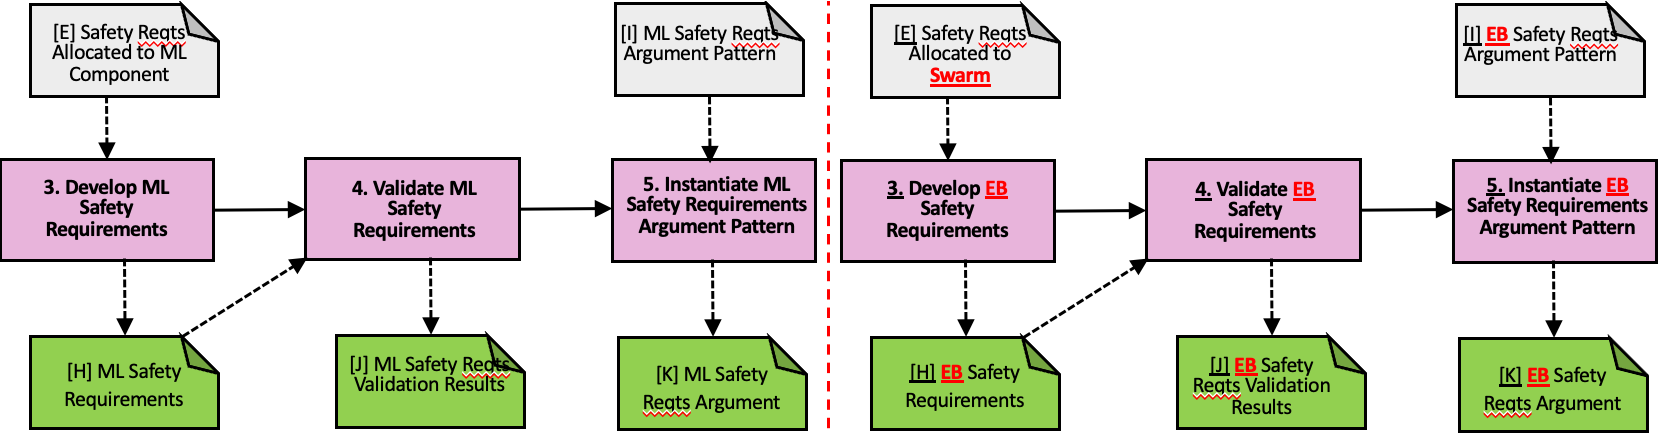
\includegraphics[width=1.0\textwidth]{figures/amlas-a-stage2.png}
	\caption{Adapted AMLAS emergent behaviour safety requirements assurance process (right).}
	\label{amlas-a-stage2}
\end{figure*}

\subsection{Stage 3: Data Management} \label{framework-stage3}
% \noindent \textbf{\textit{[Lead:  WP5]}}\\ 
% \noindent\textbf{\textit{Author Guidelines: 900–1800 words / 1–2 pages (maximum); \\Format/structure: Describe adapted AMLAS activities, inputs and outputs using cloakroom case study examples. Activities: 6, 7, 8; Inputs: H; Outputs: L0, L1, M, N, O, P, Q, S}}\\
% See Fig.~\ref{amlas-a-stage3}
% \begin{figure*}
% 	\centering
% 	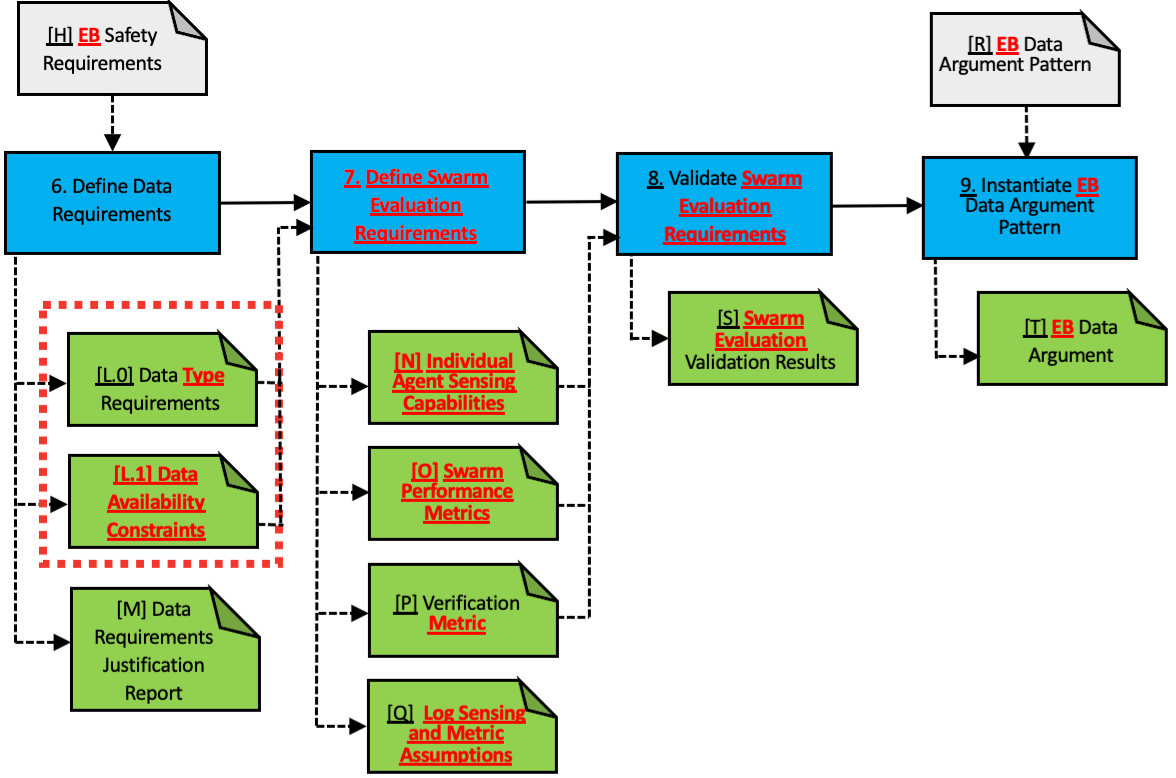
\includegraphics[width=1.0\textwidth]{figures/amlas-a-stage3.png}
% 	\caption{Adapted AMLAS data management process.}
% 	\label{amlas-a-stage3}
% \end{figure*}

In the case of designing emergent behaviours data plays a vital role, though one that differs from the machine learning applications AMLAS was initially designed for. In order to address this difference, the following activities and outputs have been adjusted to take into account the swarm behavioural design process and the added complexities that come with multiple agents interacting with one another.

\begin{figure*}
	\centering
	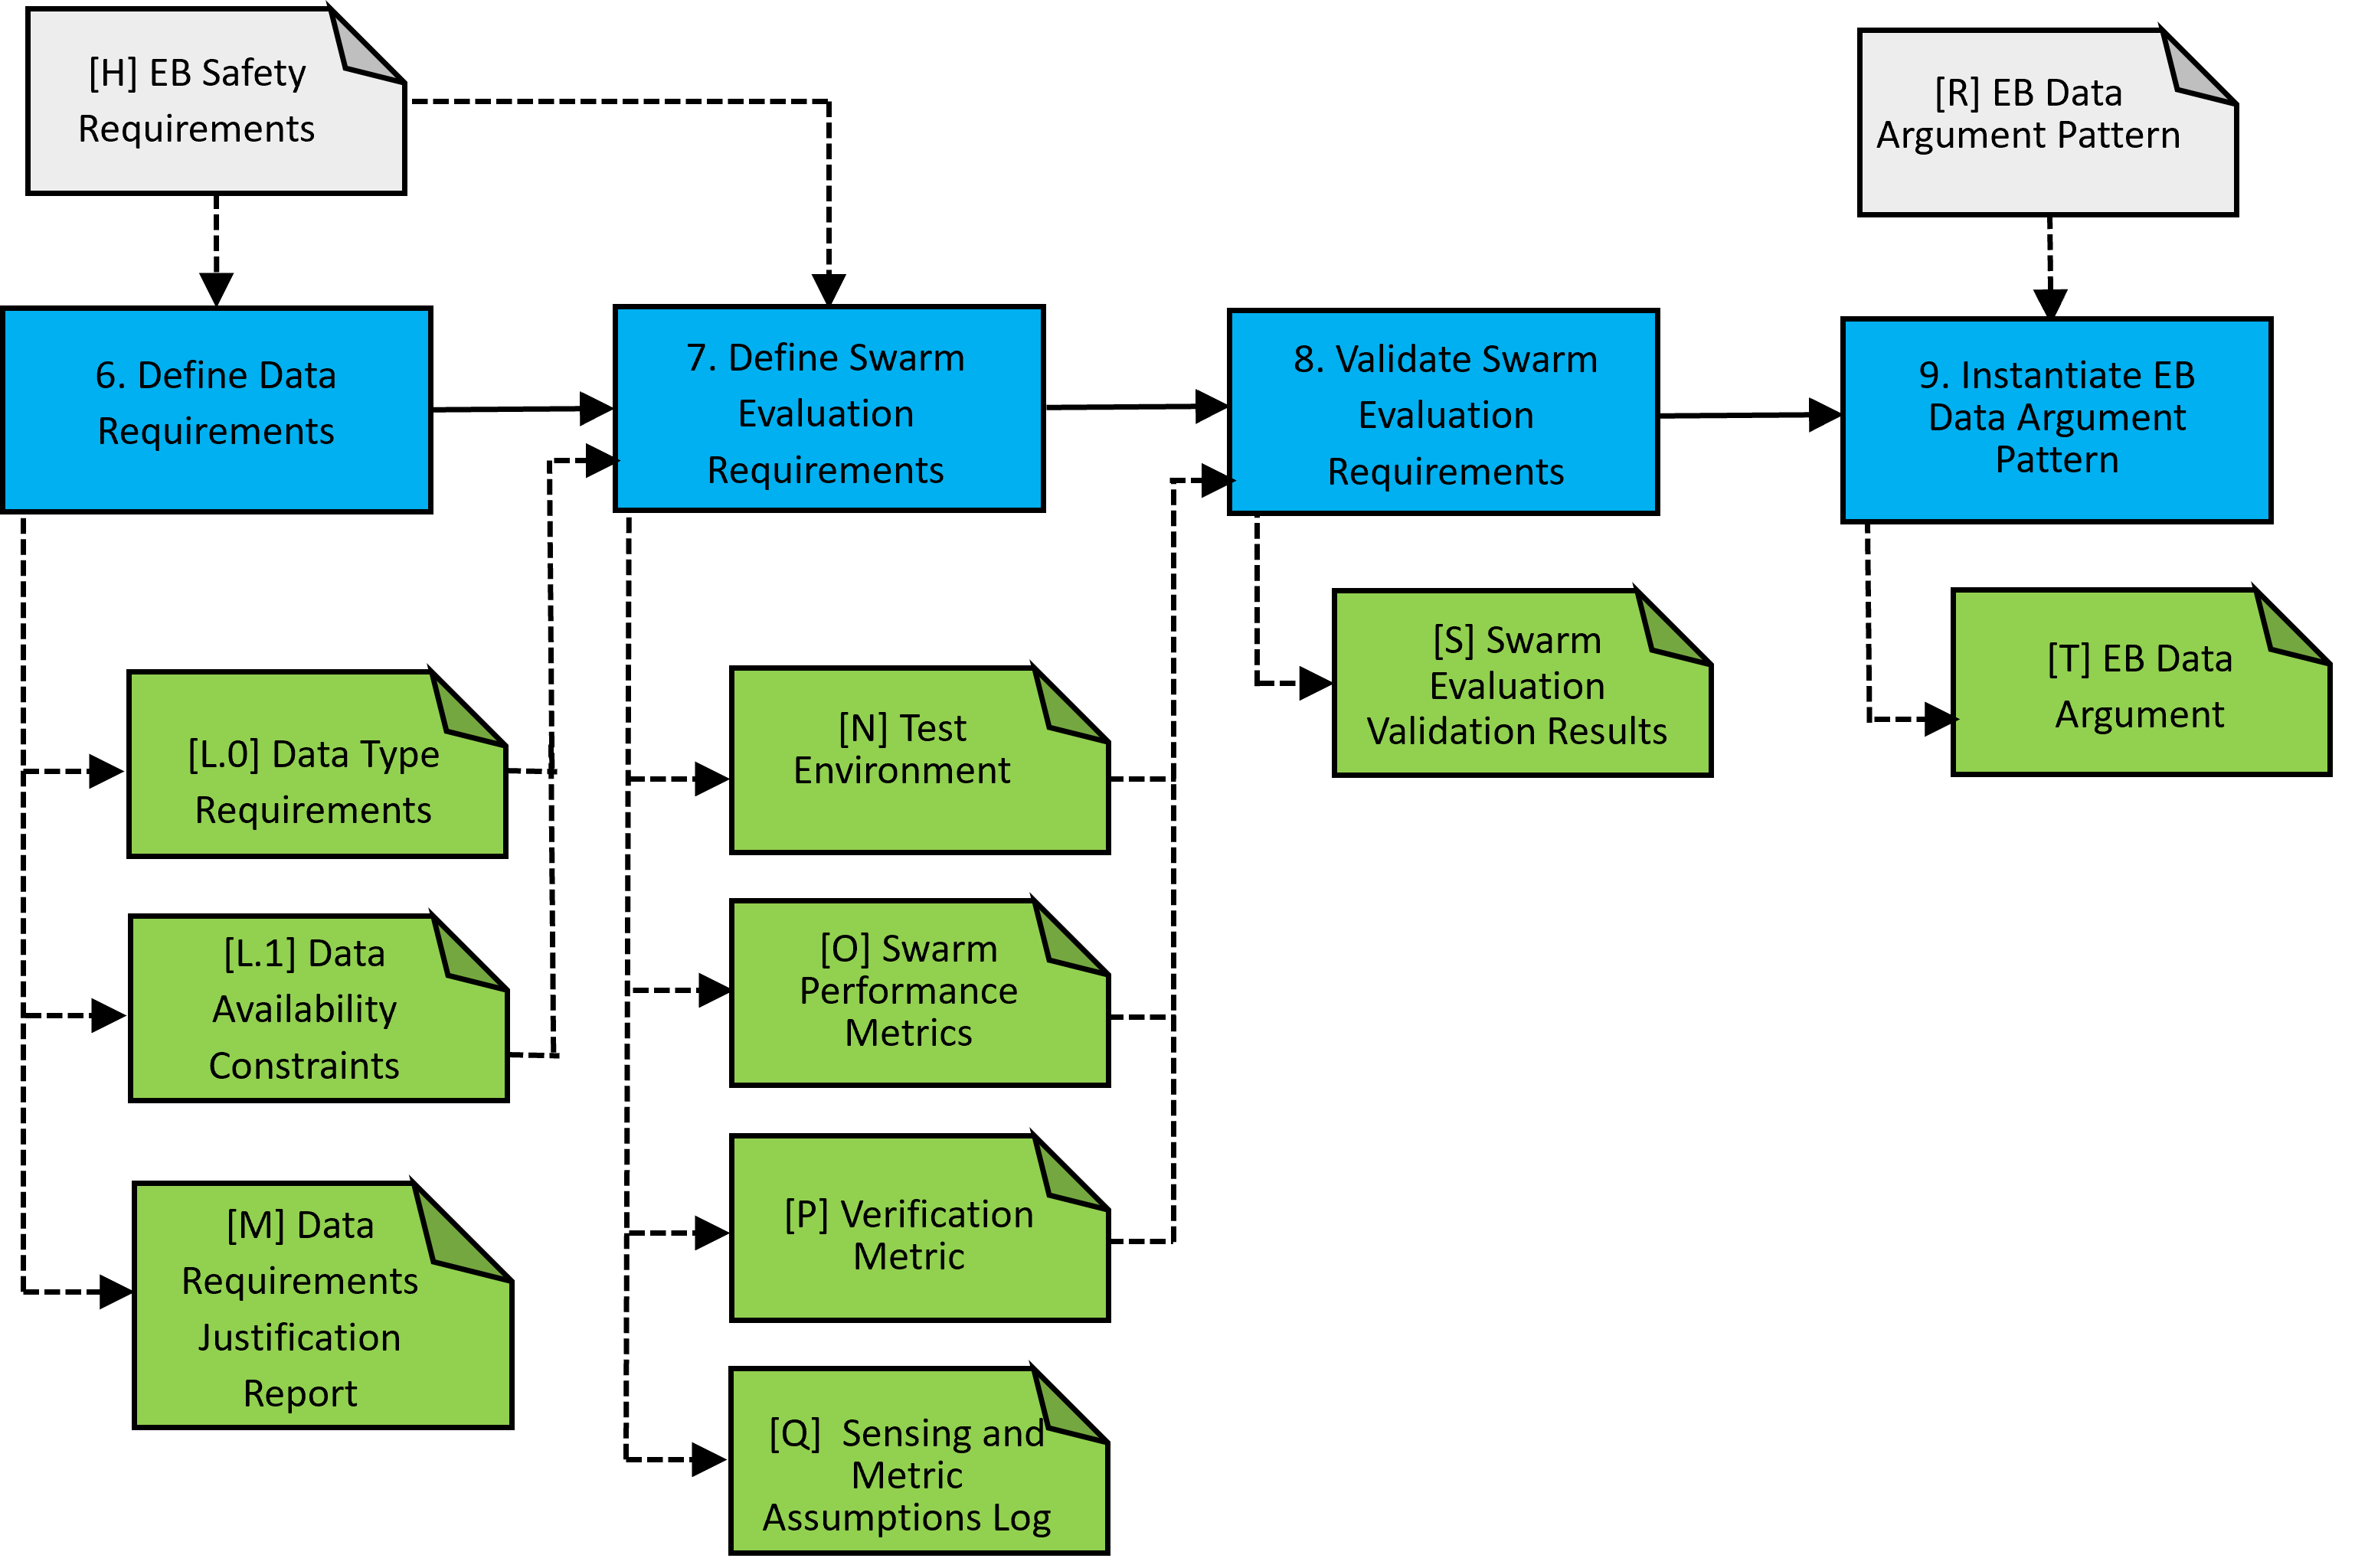
\includegraphics[width=1.0\textwidth]{figures/Stage3_DM.png}
	\caption{Adapted AMLAS data management process.}
	\label{amlas-a-stage3}
\end{figure*}

\subsubsection*{Activity 6. Define Data Requirements}

% AMLAS - This activity requires as input the ML safety requirements ([H]) as described in Stage 2 and, from these requirements, data requirements ([L]) shall be generated. Of particular interest in the development of data requirements are those safety requirements which pertain to the description of the system environment.

In our adaptation of activity 6 we take the emergent behaviour safety requirements [H] outlined in Stage 2 as an input. These safety requirements guide the data requirements in this activity, feeding into the data specification that we outline here. Unlike the original AMLAS framework, we have split the data requirement [L] into two multi-agent focused requirements: [L.0] data type requirements and [L.1] data availability constraints.

\paragraph*{[L.0] Data Type Requirements}

This elements focus on the relevance, completeness, accuracy, and balance of the information that will be used to construct the swarm behaviour and will be subsequently used to test the emergent behaviour of the system prior to its deployment.

The relevance of the data used in the development of the emergent behaviour specifies the extent to which the test environment must match the intended operating domain into which the model is to be deployed.

The completeness of the data specifies the conditions under which we test the behaviour algorithm i.e. the volume of experiments or tests that will be run, the variety of tests executed, and the diversity of environments expected to be used in the testing process.

Accuracy in this context relates to the parameters defining the performance of the swarm systems primary function. For example, what constitutes a delivery in a logistics scenario, or under what conditions would an area be considered explored in a surveying mission.

Balance, outside of a machine learning use case, refers the balance of the trials executed in the testing process of the emergent behaviour algorithm. By considering balance, we expect the number of tests conducted for individual failure modes or environment types to be justified, ensuring that there is not an unrealistic bias in testing towards a particular scenario.

In Table \ref{tab:L0} we list each of the requirement focuses considered in this output and provide respective examples of swarm data requirements.

\begin{table}[H]
    \centering
    \begin{tabular}{p{2cm} p{6cm}}
        \textbf{Requirement} & \textbf{Example} \\
        \hline
        Relevance & All simulations shall include environments with different ranges of incline between 0-20\textdegree.\\
        \hline
        & All simulations shall be conducted in a dry environment.\\
        \hline
        & All simulations shall include floors with step increases that are $\leq$ 0.5 cm.\\
        \hline
        Completeness & All simulations shall be repeated to include fault injections representative of full communication faults.\\
        \hline
        & All simulations shall be repeated a sufficient number of times to ensure results are representative of typical use.\\
        \hline
        & All simulations shall be repeated in multiple environments representative of those expected in real-world use of the system.\\
        \hline
        & All simulations shall include sufficient range of robot density levels within the scope of the operational domain.\\
        \hline
        Accuracy & All boxes shall only be considered ‘delivered’, if all four of the boxes’ feet are positioned within the delivery zone.\\
        \hline
        & All boxes shall only be considered ‘delivered’, once they are no longer in direct contact with a swarm agent.\\
        \hline
        Balance & All simulations shall be repeated equally across all test environments.\\
        \hline
        & All simulations shall be repeated equally across all test environments.\\
    \end{tabular}
    \caption{Requirement focuses for output [L.0] with representative examples from the cloakroom use case.}
    \label{tab:L0}
\end{table}

\paragraph*{[L.1] Data Availability Constraints}

With the introduction of multiple agents comes the issue of data availability. Distributed communication is a key feature found in emergent systems. As such, it is crucial to define how much information each agent is expected to hold, how easily data may transfer between agents, and across what range agents should be able to transfer information between one another. We present a list of feasible constrains with representative examples in Table \ref{tab:constraints}.

\begin{table}[H]
    \centering
    \begin{tabular}{p{2cm} p{6cm}}
         \textbf{Constraint Type} & \textbf{Example}  \\
         \hline
         Storage capacity & The swarm agents shall have a maximum of 2 GB of information stored on board at any point in time. \\
         \hline
         Available sensors & The swarm agents shall only have access to environmental data deemed feasibly collectable by infrared sensors positioned radially every 30 degrees. \\
         \hline
         Communications Range & The swarm agents shall only have access to other agent data when within communications range of 5 meters. \\
         \hline
         Operator feedback & The swarm agents shall only share information with non-agent’s (e.g. operator terminal) when within communications range of 5 meters.
    \end{tabular}
    \caption{Swarm data constraints for output [L.1] with representative examples from the cloakroom use case.}
    \label{tab:constraints}
\end{table}

\paragraph*{[M] Data Requirements Justification Report}

This report remains mainly unchanged from the traditional AMLAS framework. This report acts as an assessment of the data requirements, providing analysis and explanation for how the requirements and constraints (outlined in [L.0] and [L.1]) address the emergent behaviour safety requirements specified in [H].

\subsubsection*{Activity 7. Define Swarm Evaluation Requirements}

Taking the outputs [L.0] and [L.1] from the activity 6, the evaluation requirements take into account how the emergent behaviour of the swarm will be assessed, specifying the testing environment and the metrics comprising the test results.  

\paragraph*{[N] Test Environment}

This output takes into consideration the requirements specified in activity 6 and defines the environment in which the emergent behaviour will be tested. In most cases this will be multiple simulation environments featuring diverse sets of terrain, environmental conditions and obstacle configurations. There may also be instances in which this test environment is specified as a physical environment operating under laboratory conditions, with a hardware systems acting as a test bed to observe designed behaviours.

\paragraph*{[O] Swarm Performance Metrics}

The performance metrics specified in this activity are used to quantify how well the system is performing. While there may be multiple performance metrics, these metrics should be defined with respect to the primary function of the swarm system. Metrics that might feature in this output could include: the delivery rate in a logistics scenario, rate of area coverage as well as the efficiency of said coverage in an exploration task, or the response time in a disaster scenario.

\paragraph*{[P] Verification Metric}

These metrics should be derived from the safety requirements [H] specified in Stage 2. These metrics are intended to be used as the criteria for success within the verification process. Examples of these metrics might include: the swarm density, maximum collision force experienced by agents, or the average speed of all agents at a given time.

\paragraph*{[Q] Sensing and Metric Assumptions Log}

Much like the data log used within the traditional AMLAS framework, this log serves as a record of the details and decisions made in activities 6 and 7. This log should contain details of the choices made when producing the Test environment [N], Swarm Performance Metrics [M] and the Verification Metric [P].

\subsubsection*{Activity 8. Validate Evaluation Requirements}

Taking into account outputs [N], [O] and [P] from activity 7, this activity aims to validate these components with respect to the requirements specified in activity 6. Should any discrepancies exist between the data requirements and the evaluation requirements, they should be justified appropriately and recorded in output [S] Swarm Evaluation Validation Results.

\subsection{Stage 4: Model Emergent Behaviour} \label{framework-stage4}
\noindent \textbf{\textit{[Lead:  WP5]}}\\ 
\noindent\textbf{\textit{Author Guidelines: 900–1800 words / 1–2 pages (maximum); \\Format/structure: Describe adapted AMLAS activities, inputs and outputs using cloakroom case study examples. Activities: 10, 11; Inputs: H, N, O; Outputs: Candidate EB Algorithm, U, V, X}}\\\\
See Fig.~\ref{amlas-a-stage4}
\begin{figure*}
	\centering
	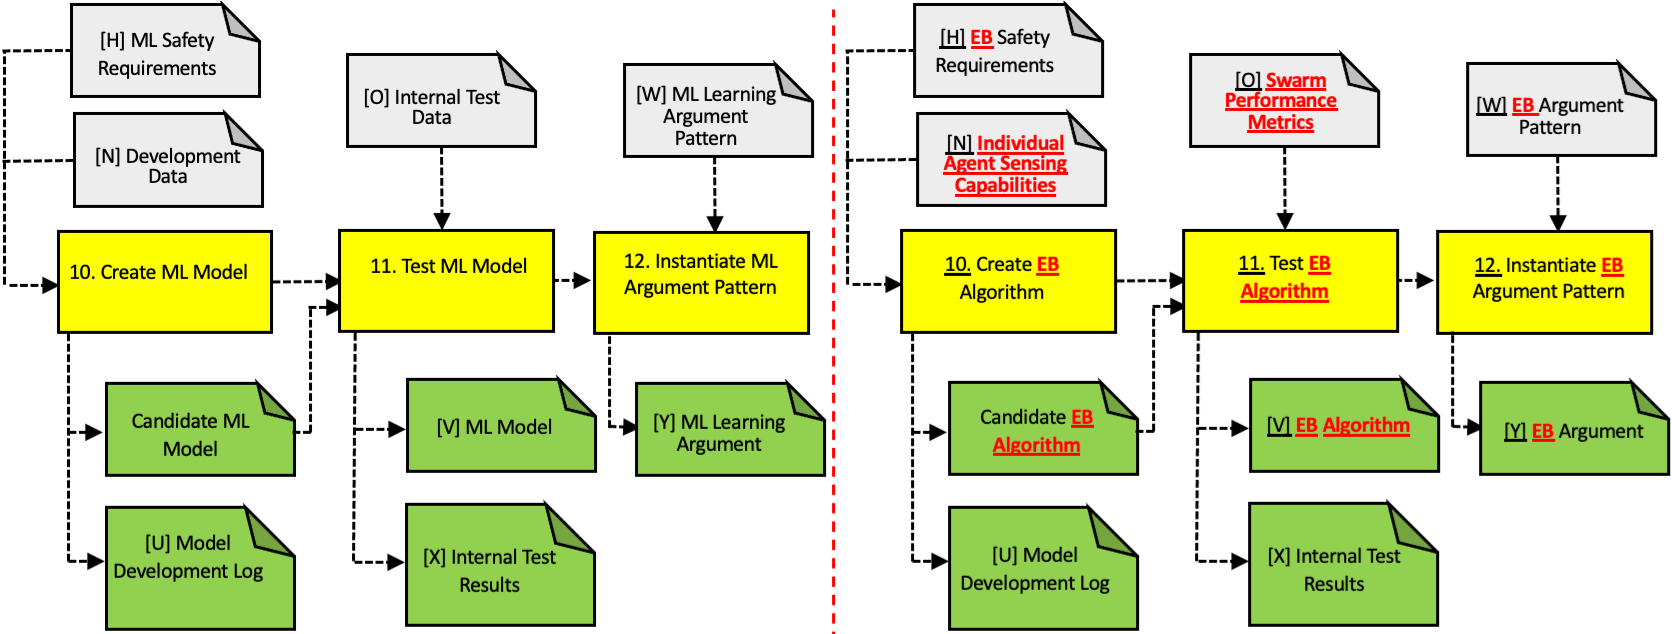
\includegraphics[width=1.0\textwidth]{figures/amlas-a-stage4.png}
	\caption{Adapted AMLAS model learning process (right).}
	\label{amlas-a-stage4}
\end{figure*}

\subsection{Stage 5: Model Verification} \label{framework-stage5}
\noindent \textbf{\textit{[Lead:  WP4]}}\\ 
\noindent\textbf{\textit{Author Guidelines: 900–1800 words / 1–2 pages (maximum); \\Format/structure: Describe adapted AMLAS activities, inputs and outputs using cloakroom case study examples. Activities: 13; Inputs: H, P, V; Outputs: Z, AA}}\\
See Fig.~\ref{amlas-a-stage5} and Fig.~\ref{amlas-a-testbench}.	
\begin{itemize}
	\item Test bench for swarms
	\item Probabilistic verification ideas
	\item Simulation-based testing
	\item Verifiability?
\end{itemize}
\begin{figure*}
	\centering
	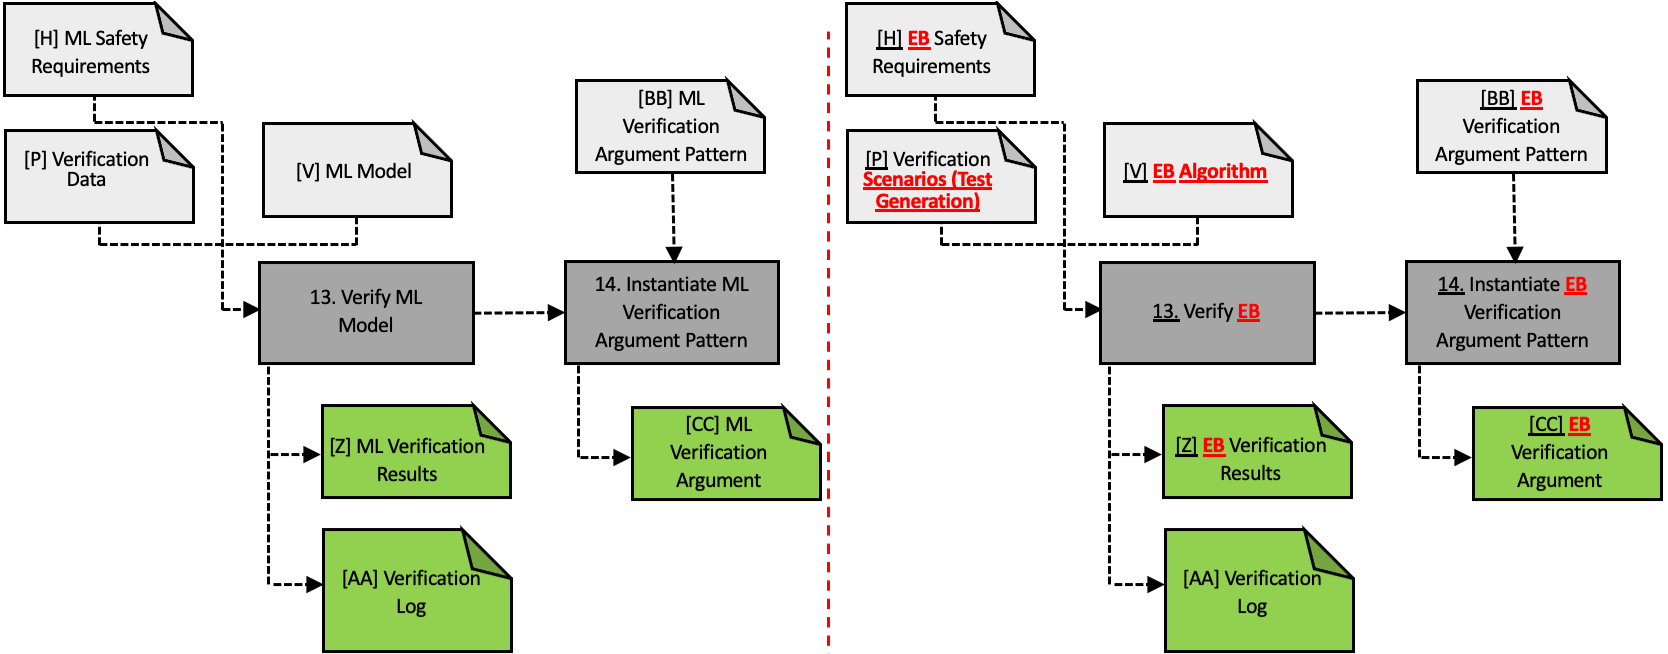
\includegraphics[width=1.0\textwidth]{figures/amlas-a-stage5.png}
	\caption{Adapted AMLAS verification assurance process (right).}
	\label{amlas-a-stage5}
\end{figure*}
\begin{figure*}
	\centering
	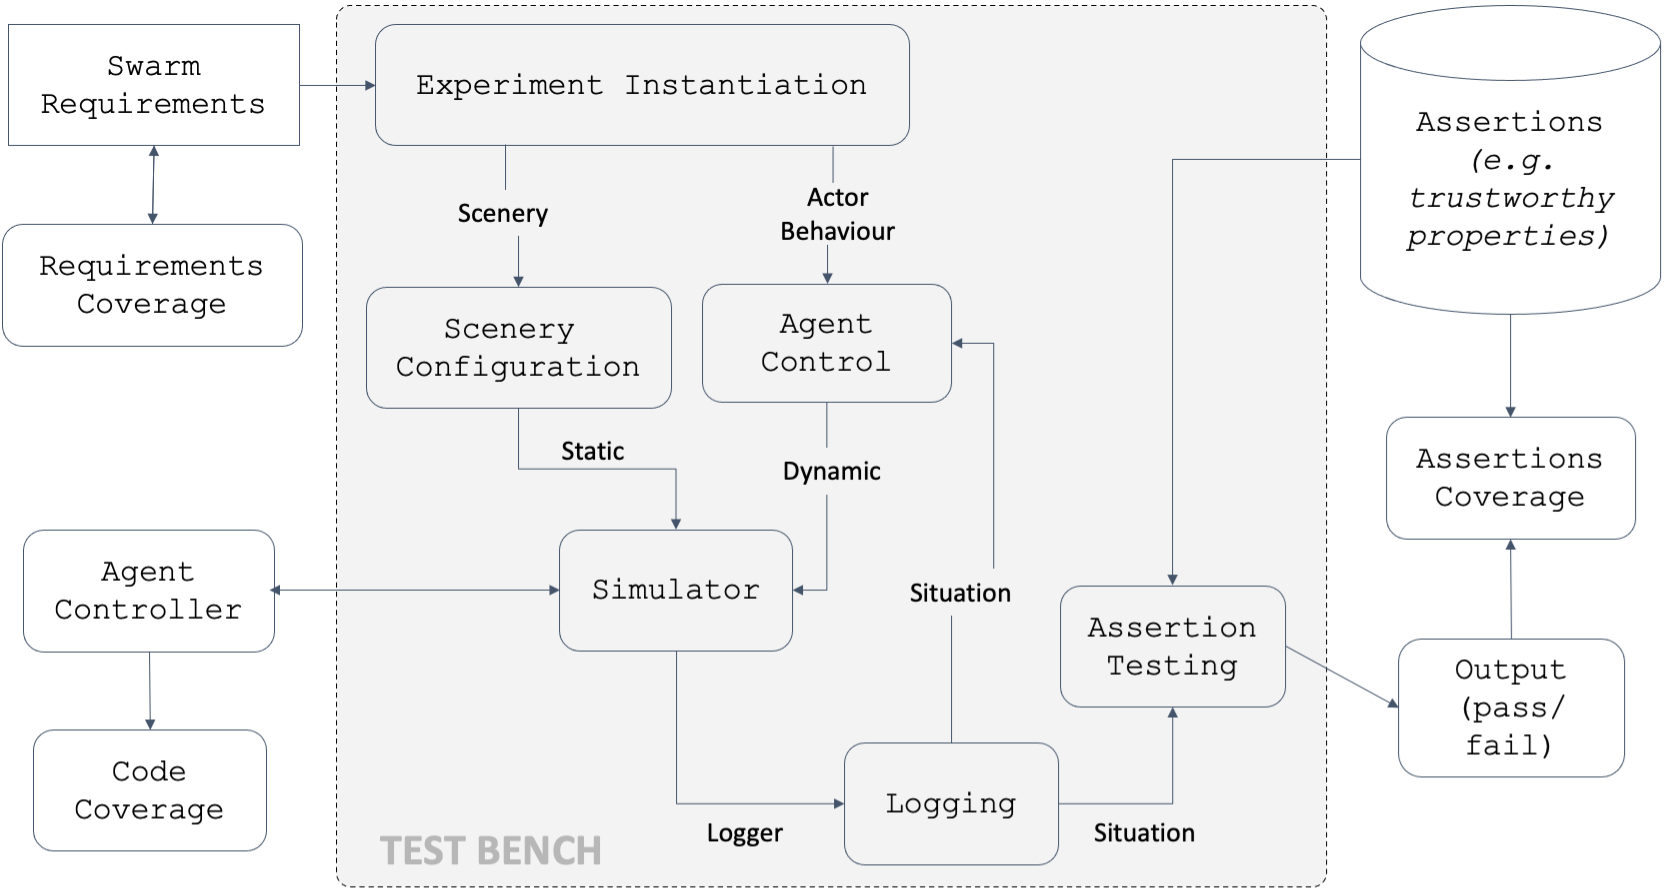
\includegraphics[width=1.0\textwidth]{figures/verification-testbench.png}
	\caption{Adapted AMLAS verification assurance process: test bench.}
	\label{amlas-a-testbench}
\end{figure*}

\subsection{Stage 6: Model Deployment} \label{framework-stage6}
\noindent \textbf{\textit{[Leads:  WP4 \& WP5; Additional: WP3]}}\\ 
\noindent\textbf{\textit{Author Guidelines: 900–1800 words / 1–2 pages (maximum); \\Format/structure: Describe adapted AMLAS activities, inputs and outputs using cloakroom case study examples.\\ 
\noindent WP5 = (Activities: 15, Inputs: V, A, B, C, D, Outputs: DD), \\
\noindent WP4 = (Activities: 16, Inputs: EE, Outputs: FF), \\
\noindent WP3 = (Regulatory Considerations – 675 words / 0.75 page maximum)}}\\
See Fig.~\ref{amlas-a-stage6}
\begin{figure*}
	\centering
	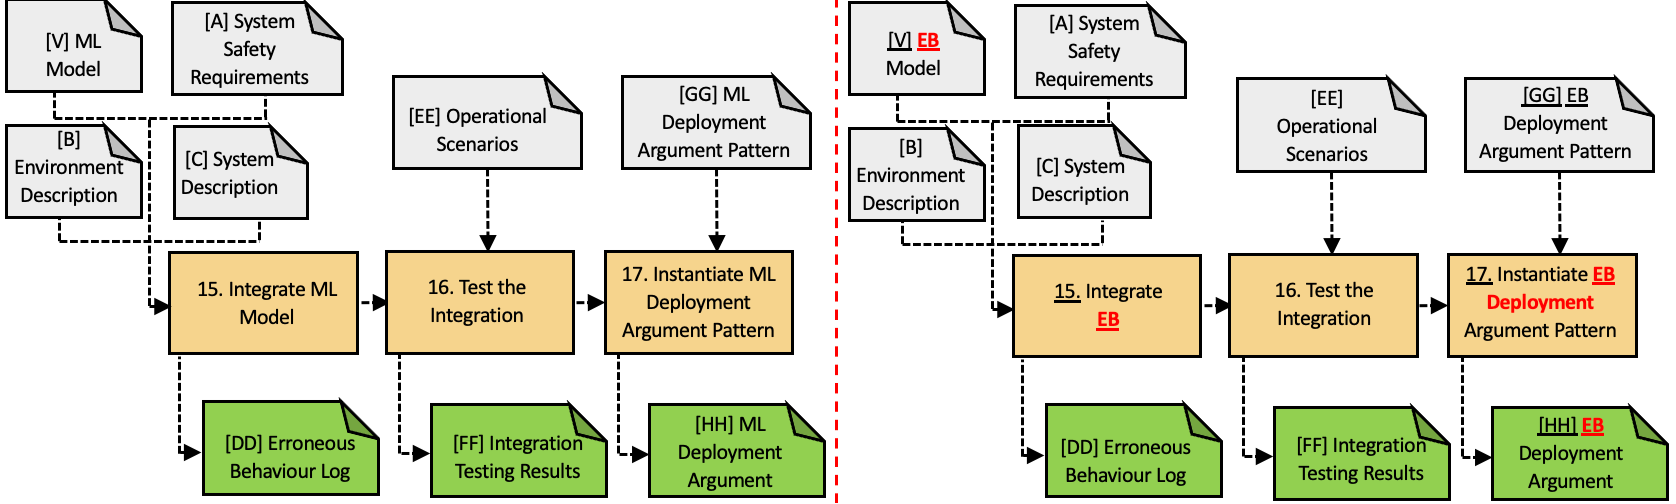
\includegraphics[width=1.0\textwidth]{figures/amlas-a-stage6.png}
	\caption{Adapted AMLAS model deployment assurance process (right).}
	\label{amlas-a-stage6}
\end{figure*}



%\subsection{Stage 7: Assurance Case}
	
\section{Discussion and Conclusions} \label{discussion-conclusions}

\section*{Acknowledgments}
The work presented in this paper has been supported by the UK Engineering and Physical Sciences Research Council (EPSRC) under the grant [EP/V026518/1].

{\appendices
\section*{Appendix A. Supplementary Material}
The supplementary material associated with this article can be found online at (https://www.).


\bibliographystyle{IEEEtran}
\bibliography{AssuranceFWK-Swarms-Bibliography}

\newpage

\vfill

\end{document}


